\section{Building the Engine}

In this section we detail all the work that has been done on building our model which is the backbone of our engine. We start by describing the intuition behind using Natural Language Processing, then introduce N-gram models as our NLP technique of choice and close by describing how we incorporated that into our completion engine.

\subsection{Token Analysis}
Prior research in computer networking hints that we should expect network configurations to share a common set of tokens. As Hindle,\textit{et al.} 2012~\cite{naturalness} pointed out, regularities in bodies of texts can be easily exploited by NLP techniques. We hope to find and use such regularities in network configurations to generate suggestions.\\

In~\cite{complexity} researchers identified a few key design decisions commonly made by network operators. Network configurations are designed to be homogeneous as a means of easy maintenance, where some operators start off with common configuration templates with varying parameters. They may then tweak these templates to achieve specialized routing roles if needed. Thus one can posit that configurations across devices in a given network may share a lot of the same tokens, subnets and sometimes even complete stanzas (such as Access Control Lists).\\ 

To confirm our hypothesis, we took configurations from a large university network and split up each configuration file into a list of tokens. Tokens included all keywords and subnets with punctuation and newline characters stripped off. For every file we then plotted the percentage of tokens that exist in other router configuration files.

\begin{figure}[H]
	\centering
	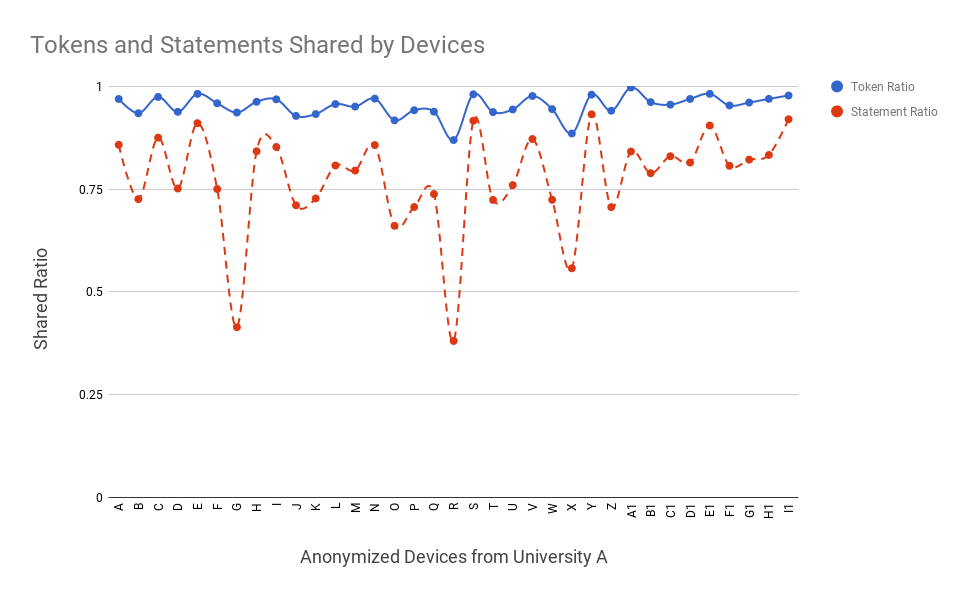
\includegraphics[width=\textwidth]{chart.png}
	\caption{The plot shows how many tokens and statements a router configuration holds in common with the rest of the network. The data was taken from a large research university.}
\end{figure}

Our results show that most of each file could be rebuilt from existing statements in routing configurations due to the amount of tokens they share. Given our results, and the observations made by~\cite{complexity} about how networks are configured, we can confidently hypothesize that most token suggestions can be generated from analyzing other existing configurations. This effectively makes all router configuration histories a part of the search space for our NLP model. 

\subsection{N-gram Models}

Once we were confident that token regularities existed in network configurations, we began exploring NLP techniques to make use of token histories. As we mentioned in Section 2.2, we have decided on n-gram models as a basis of our engine. Here we briefly describe the theory behind these models. 

Consider a sequence of tokens in a body of text (in our case, network configurations). We can statistically model how likely tokens are to follow other tokens. We accomplish this by calculating the conditional probabilities of certain tokens appearing in the text. Given a sequence of tokens $a_1,a_2,a_3,...,a_n$, we can calculate the probability of $a_2$ occurring given that $a_1$ has already occurred i-e $p(a_2 | a_1)$. We continue by calculating the probability of $a_3$ given $a_2$, and so on. Since we looked at two tokens at a time, this is called a bigram model. More generally, predicting how likely a token is to show up based on the previous $n-1$ tokens is called an n-gram model. In our work, we plan to use bigram and trigram models.

\subsection{Likelihood Estimators} 

The probabilities for suggesting a token pair are estimated by using some scoring function. Often a function may simply count the frequency by which a given pair occurs in the training data and calculate the probability as a ratio of frequency of the pair to the total token count. However, we utilize likelihood estimators as they provided good accuracies for Hindle,\textit{et al.} and have been known to work well for n-gram models~\cite{manning}.

Likelihood ratios are one approach to hypothesis testing. The two hypotheses in our case are:

\begin{center}
Hypothesis 1: $P(w_2|w_1) = p = P(w_2|\neg w_1)$ \\
Hypothesis 2: $P(w_2|w_1) = p_1 \neq p_2 = P(w_2|\neg w_1)$	\\	
\end{center}

A likelihood estimator is simply a number that tells us how much more likely one hypothesis is than the other. They also have an added advantage of generally being more appropriate for sparse data than other tests. Our system internally uses the Manning and Schutze (5.3.4) version of likelihood estimators~\cite{manning}.


\subsection{Model Construction}

N-gram models provided us with a strong foundation on which we could build a specialized completion engine. We developed a program in Python which reads in configuration files and builds a bigram model, using the NLTK package~\cite{nltk}. NLTK also allows us to easily incorporate likelihood ratios as a means of scoring the bigrams. Our script was run on sample configurations from the ARC package~\cite{arc}. These configurations are simple in nature but mimic what deployed network configurations would look like. Each set of configurations emulates a small network employing a different routing policy or design. This allows for a wide breadth of network configuration types to be considered for our model.\\ 

Next, we incorporated some preprocessing steps to clean up the data. Since IP addresses and subnets tend to vary a lot and add noise to the data, we replaced them with placeholders. In Section 4, we consider other approaches to help suggest IP addresses. Additionally, our initial analysis showed that the engine was trying to predict what the user would enter after a complete configuration statement. This greatly affected our accuracies, and thus we altered our model to only suggest tokens that appear on the same line.\\

[MODEL EVALUATION]

To test the accuracy of our model, we perform Leave One Out (LOO) Cross Validation. This form of cross validation involves using one observation as the validation set and the remaining observations as the training set. This is repeated for all combinations of training sets, allowing every observation to act as a validation set. For our analysis an observation is one set of configurations. For example, consider five sets of configurations: A through E. We pick A as the validation set and train the model on all other configurations. Our program will now "walk through" rebuilding configuration A, starting from the first keyword. At every step, we invoke our model and compare our predictions against the actual tokens in A. If the model generates the correct prediction within the top three results, we mark a token completion to be successful.\\
 
\begin{figure}[H]
	\centering
	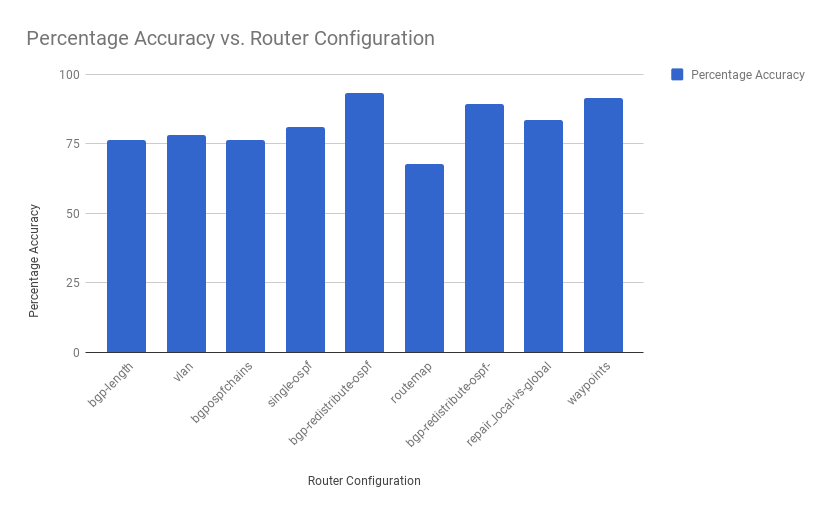
\includegraphics[width=\textwidth]{model_analysis.png}
	\caption{The bar charts show the accuracy of the model for each set of network configurations used as the validation set.}
\end{figure}
Since we had 10 sets of configurations at our disposable, we performed 10 LOOs and took the average of the accuracies for a final accuracy measure. Initially, without any preprocessing and subnet removal, we observed a maximum accuracy of 85\% and an average of 65\%. Our results in the figure above are after preprocessing the data and we now see accuracies as high as 93\%, and an average of 81\%. These results are very promising as we saw a significant jump in accuracy from simple refinements to the model. We are thus optimistic about trying new approaches for further improving accuracies that we describe in the next section.